% Разрешение 16x9
\documentclass[english,russian,aspectratio=169]{beamer}

\mode<presentation>
{
  \usetheme{Rochester}      
  \usecolortheme{beaver}
  \usefonttheme{default}
  \setbeamertemplate{navigation symbols}{}
  \setbeamertemplate{caption}[numbered]
}

\usepackage[T2A]{fontenc}
\usepackage[utf8]{inputenc}
\usepackage[english,russian]{babel}
\usepackage{graphicx}
\usepackage{longtable}
\usepackage{subfigure}
\setbeamertemplate{footline}[frame number]

\setbeamerfont{institute}{size=\fontsize{8pt}{9pt}}
\setbeamerfont{date}{size=\fontsize{8pt}{9pt}}

\usepackage{ragged2e}
\justifying

\renewcommand{\raggedright}{\leftskip=0pt \rightskip=0pt plus 0cm}

% Цвет
\definecolor{MyGrey}{RGB}{40, 41, 35}

% Строки для титульного слайда
\title{Развитие подсистемы Linux в ОС Embox для исполнения двоичных файлов}
\author{Остроухов Антон}
% Пустая дата, иначе она будет в центре слайда
\date{}

\begin{document}
\selectlanguage{russian}
\setbeamertemplate{footline}[frame number]

% Титульный слайд
\begin{frame}[plain]
\titlepage

% '\titlepage' занимает весь слайд, поэтому поднимемся вверх
\vspace{-50pt}

% ВУЗ и Направление
\begin{center}
  \scriptsize{
    Санкт-Петербургский государственный университет
    \\[2mm]Направление 02.04.03 <<Математическое обеспечение и администрирование информационных систем>>
  }
\end{center}

\vspace{10pt}

% Руководитель, консультант, рецензент
\scriptsize{
  \textbf{Научный руководитель:} проф. каф. СП, д.ф.-м.н., проф. А.Н. Терехов
  \\\textbf{Консультант:} ассистент каф. СП А.П. Козлов
  \\\textbf{Рецензент:} генеральный директор ООО <<Ембокc>> А.В. Бондарев
}

\vspace{28pt}

% Город и год
\begin{center}
  \scriptsize{
  Санкт-Петербург
  \\2022
  }
\end{center}
\end{frame}

\begin{frame}[t]{Введение}
\begin{itemize}
    \item Разработка и поддержка ОС --- трудоёмкий процесс
    \begin{itemize}
        \item Система должна включать всё необходимое ПО
    \end{itemize}
    \item Для GNU/Linux создаётся много ПО, оно может быть полезным в других ОС
    \item Совместимость с GNU/Linux может быть реализована двумя способами
    \begin{itemize}
        \item Программный интерфейс --- ПО частично изменяется и повторно компилируется
        \item Двоичная совместимости --- возможность обрабатывать системные вызовы Linux
    \end{itemize}
    \item В ОС Embox существует совместимость на уровне программного интерфейса
    \begin{itemize}
        \item Поддержка программного интерфейса стандарта POSIX
        \item Ранее мною была адаптирована библиотека Linux Kernel Library~---\newline
        ядро Linux как библиотека
        \item Обеспечение слоя двоичной совместимости расширит множество доступного\newline
        стороннего ПО
    \end{itemize}
\end{itemize}

\end{frame}

\begin{frame}[t]{Цель и задачи}
\textbf{Цель} --- разработать для ОС Embox подсистему, обеспечивающую возможность\newline
исполнения двоичных файлов, скомпилированных для GNU/Linux

\vspace{8pt}
\textbf{Задачи}
\begin{enumerate}
    \item Провести анализ существующих подходов для выбора наиболее универсальных архитектурных решений
    \item Разработать архитектуру подсистемы двоичной совместимости с GNU/Linux, не зависящую от особенностей конкретной операционной системы
    \item На основе разработанной архитектуры реализовать подсистему для ОС Embox
    \item Провести апробацию созданной подсистемы
\end{enumerate}
\end{frame}

\begin{frame}[t]{Обзор существующих решений}
Были проанализированы решения по обеспечению слоя двоичной совместимости с GNU/Linux в FreeBSD, Windows, L4 и т.д.

\vspace{8pt}
Выделены два подхода:
\begin{enumerate}
    \item Эмуляция работы ядра Linux
    \begin{itemize}
        \item ОС готовит двоичное окружение и реализует вызовы Linux через свои
        \item Ручная реализация системных вызовов и прочие недостатки
    \end{itemize}
    \item Паравиртуализация ядра Linux
    \begin{itemize}
        \item Адаптированное ядро Linux обрабатывает системные вызовы Linux
        \item Требуется модификация ядра Linux
        \item Существующие решения слишком зависят от целевых ОС
    \end{itemize}
\end{enumerate}
\end{frame}

\begin{frame}[t]{Архитектура}
\begin{figure}[h]
\center{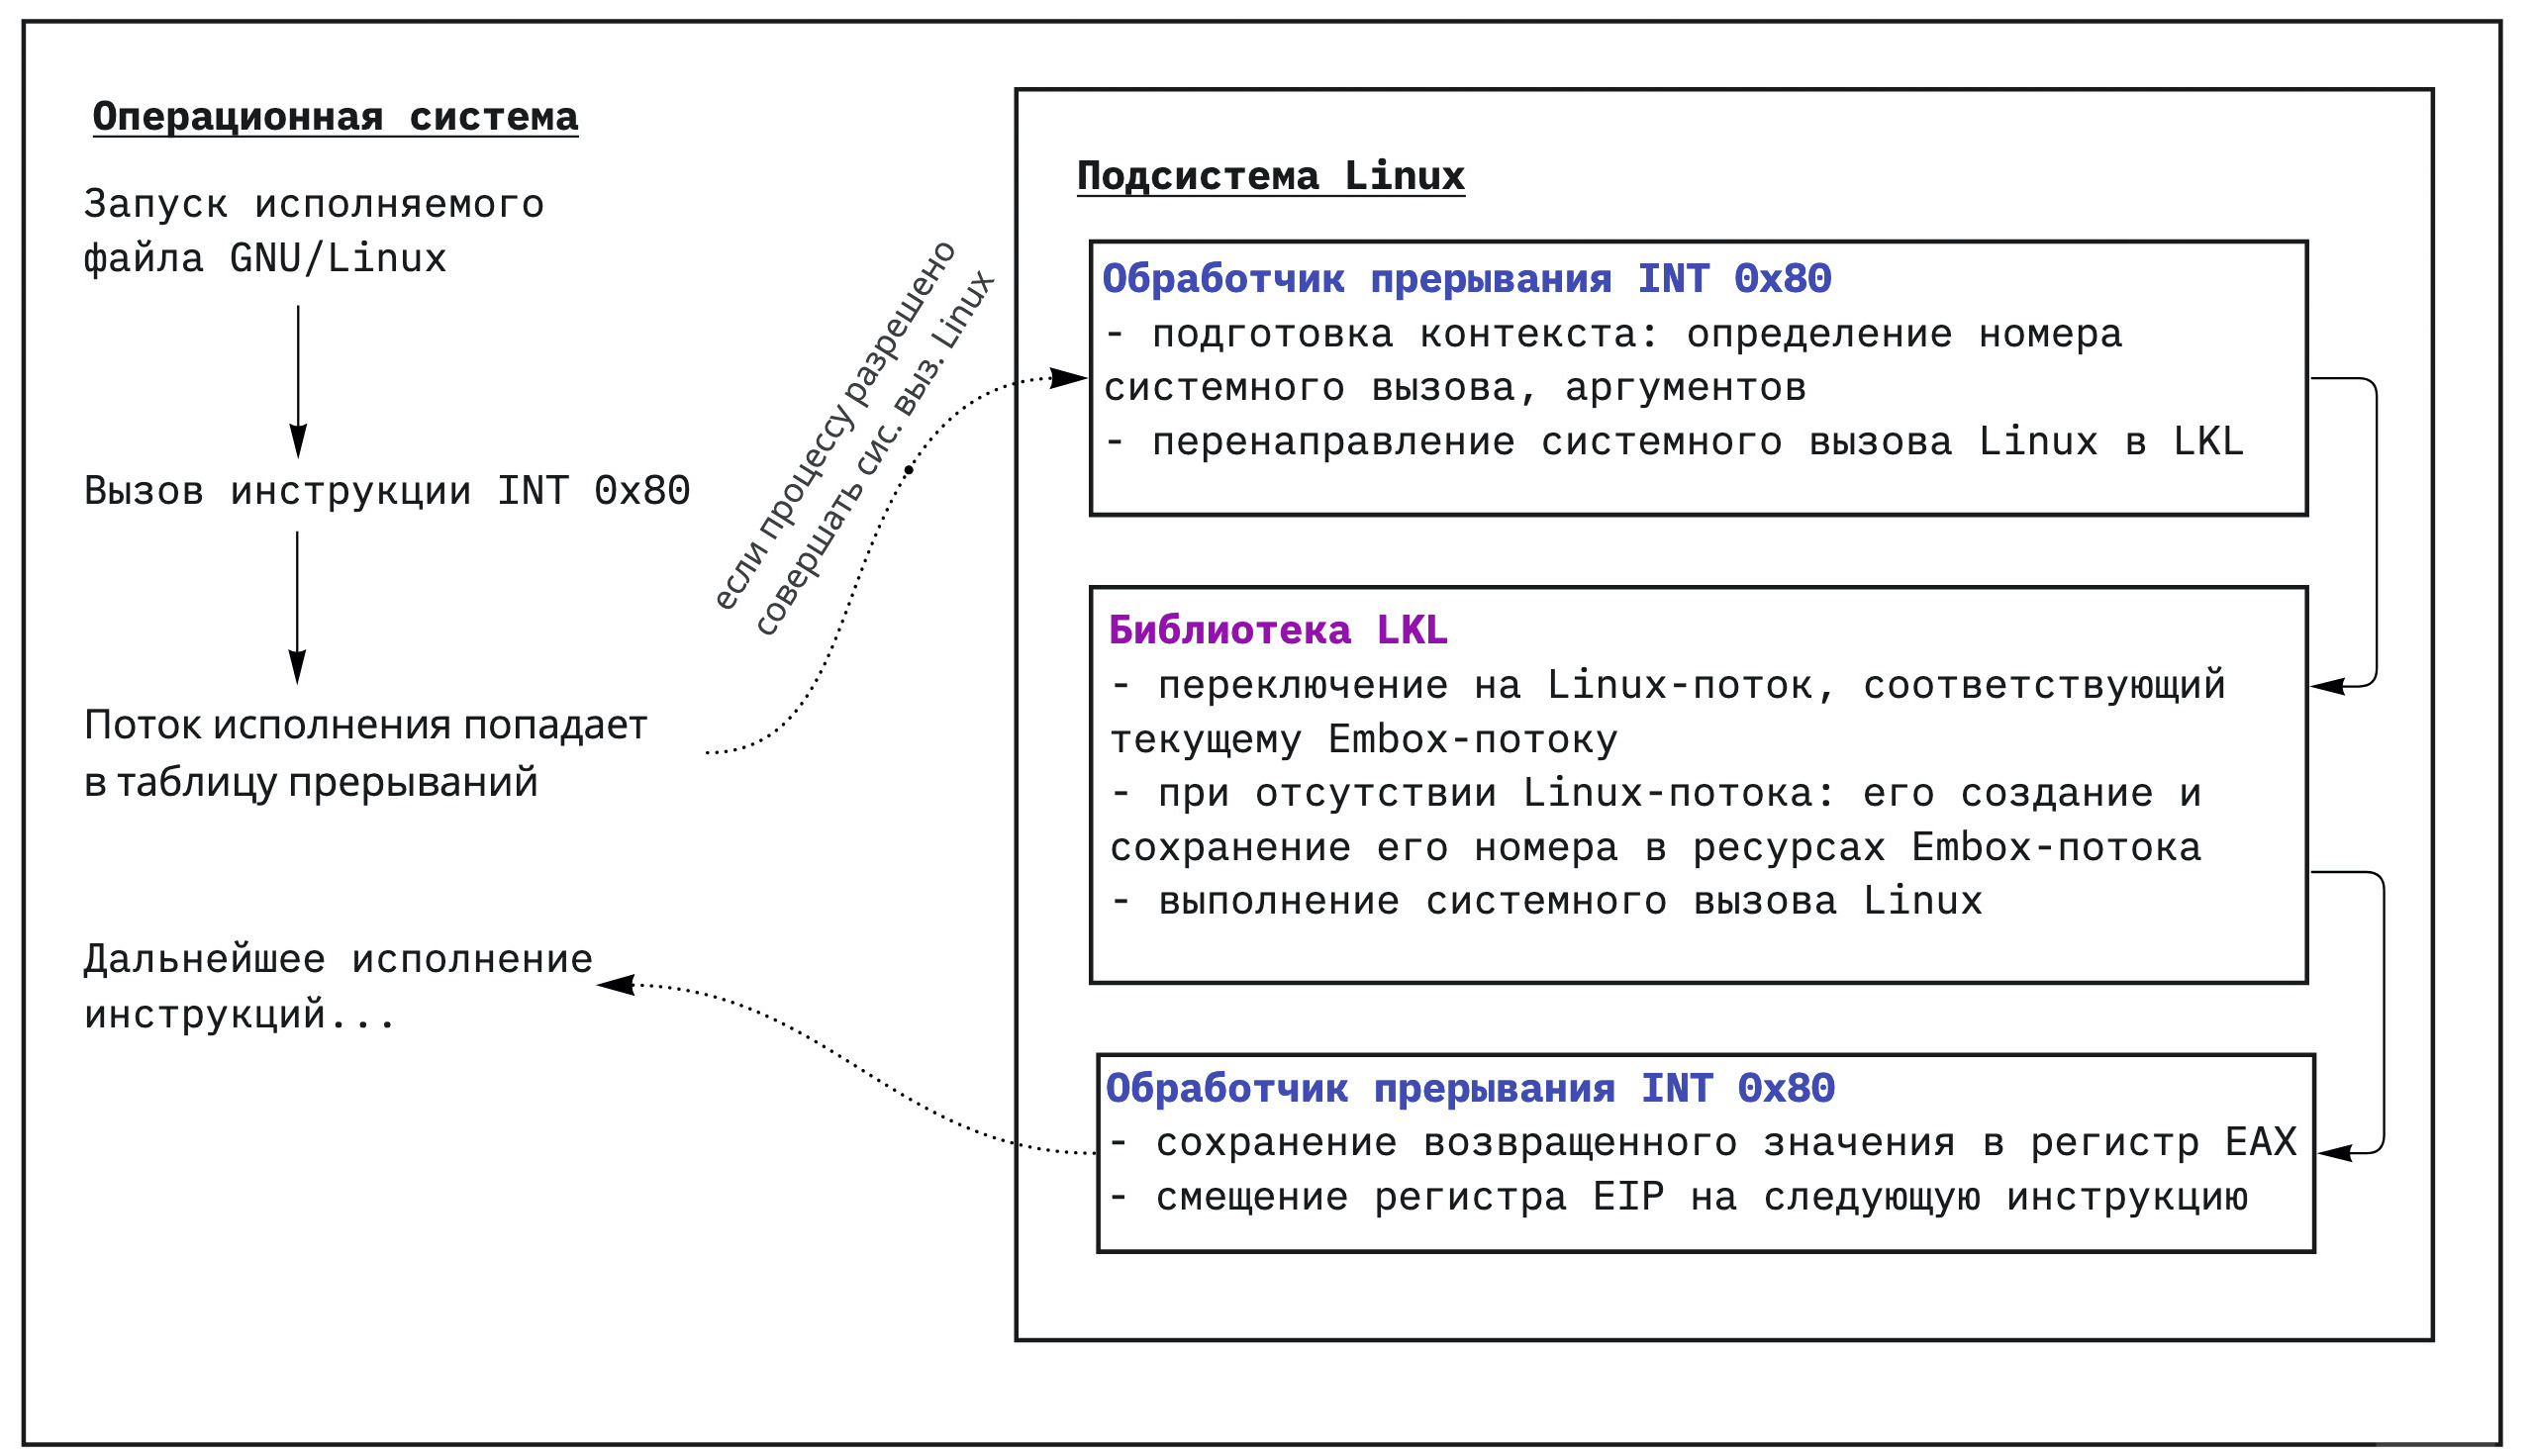
\includegraphics[scale=0.11]{pictures/Arch.jpg}}
\caption{Архитектура слоя совместимости}
\end{figure}
\end{frame}

\begin{frame}[t]{Особенности реализации}
Подсистема на основе описанной архитектуры реализована в Embox
\vspace{8pt}
\begin{itemize}
    \item Подсистема --- модуль, подключаемый на этапе сборки образа ОС Embox
    \item Инструмент загрузки сторонних программ \textcolor{MyGrey}{\texttt{load\_app}} разрешает процессу\newline
    выполнять системные вызовы Linux
    \item В контексте LKL реализовано \textit{специальное блочное устройство}, которое\newline
    выводит поток текста из LKL в терминал ОС Embox
\end{itemize}
\vspace{8pt}
Запрос на привнесение изменений в ОС Embox:\newline
\textcolor{MyGrey}{\texttt{github.com/embox/embox/pull/2561}}
\end{frame}

\begin{frame}[t]{Тестирование и апробация}
\vspace{8pt}
\begin{itemize}
    \item Реализованы упрощённые аналоги некоторых инструментов GNU/Linux,\newline
    которые были скомпонованы \textit{статически}
    \begin{itemize}
        \item Embox не поддерживает динамическую компоновку
    \end{itemize}
    \item Продемонстрирована работа с файловой системой \textcolor{MyGrey}{\texttt{procfs}}
    \begin{itemize}
        \item Реализуется в коде ядра Linux
        \item Не специфицирована, поэтому в разных ОС может отсутствовать
        \item Программы, которые зависят от подобных элементов ядра Linux, будут работать
    \end{itemize}
\end{itemize}
\end{frame}

% echo
\begin{frame}{Тестирование и апробация}
\begin{figure}[h]
\center{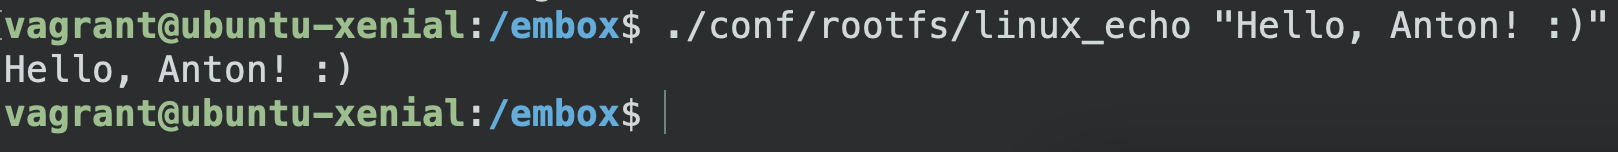
\includegraphics[scale=0.35]{pictures/linux_echo.png}}
\caption{{Исполнение \textcolor{MyGrey}{\texttt{linux\_echo} в ОС Ubuntu}}}
\end{figure}
\end{frame}

\begin{frame}{Тестирование и апробация}
\begin{figure}[h]
\center{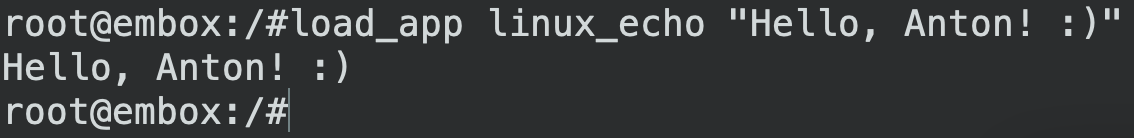
\includegraphics[scale=0.5]{pictures/embox_echo.png}}
\caption{{Исполнение \textcolor{MyGrey}{\texttt{linux\_echo} в ОС Embox}}}
\end{figure}
\end{frame}

% ls
\begin{frame}{Тестирование и апробация}
\begin{figure}[h]
\center{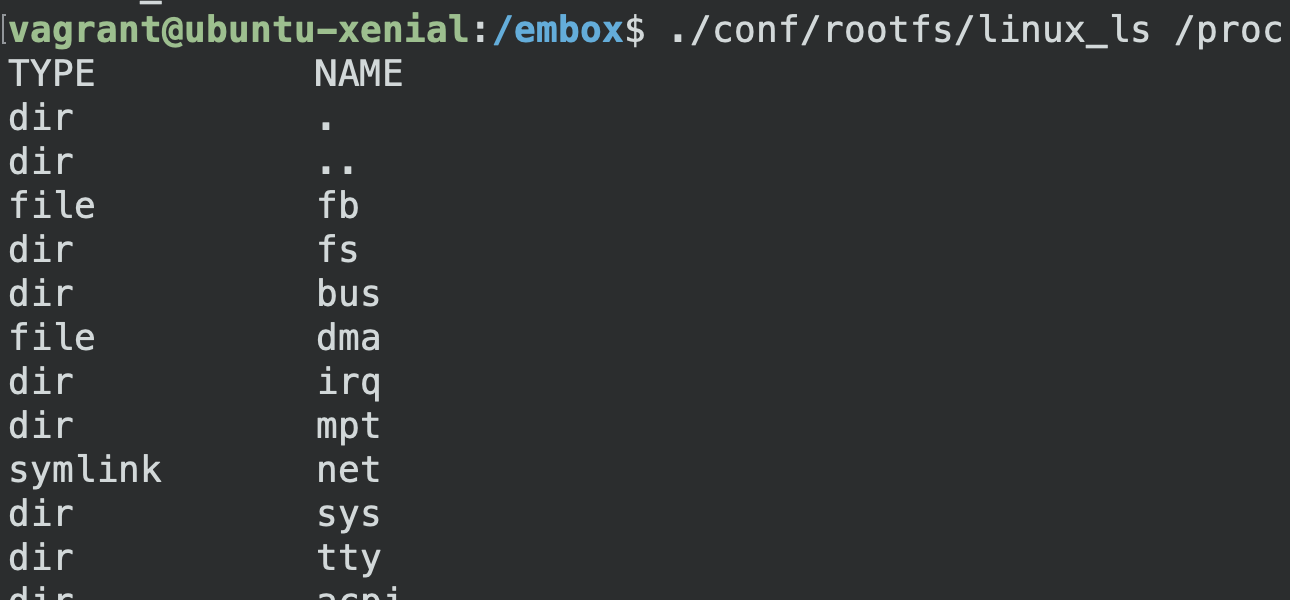
\includegraphics[scale=0.35]{pictures/linux_ls.png}}
\caption{Исполнение \textcolor{MyGrey}{\texttt{linux\_ls}} (каталог \textcolor{MyGrey}{\texttt{/proc}}) в ОС Ubuntu}
\end{figure}
\end{frame}

\begin{frame}{Тестирование и апробация}
\begin{figure}[h]
\center{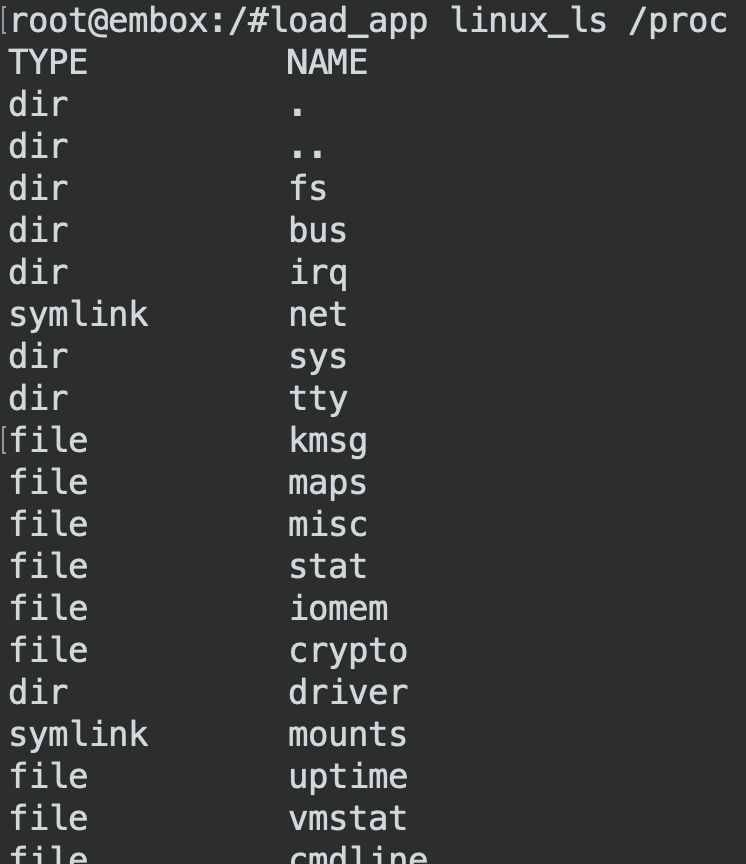
\includegraphics[scale=0.35]{pictures/embox_ls_proc.png}}
\caption{{Исполнение \textcolor{MyGrey}{\texttt{linux\_ls}} (каталог \textcolor{MyGrey}{\texttt{/proc}}) в ОС Embox}}
\end{figure}
\end{frame}

% cat
\begin{frame}{Тестирование и апробация}
\begin{figure}[h]
\center{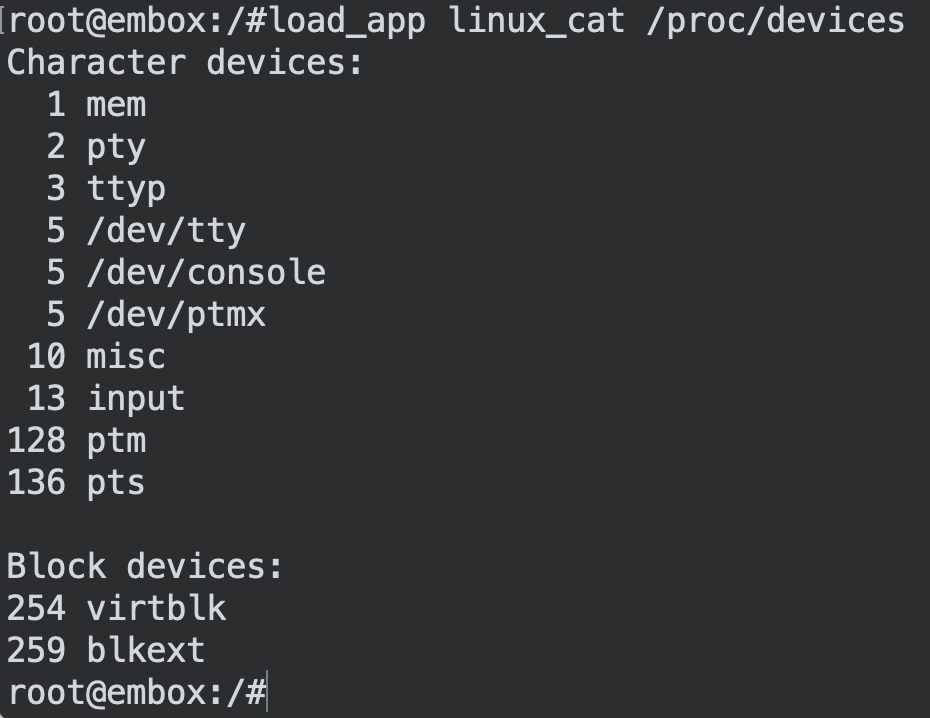
\includegraphics[scale=0.4]{pictures/embox_cat_devices.png}}
\caption{Исполнение \textcolor{MyGrey}{\texttt{linux\_cat}} (файл \textcolor{MyGrey}{\texttt{/proc/devices}}) в ОС Embox}
\end{figure}
\end{frame}

\begin{frame}{Тестирование и апробация}
\begin{figure}[h]
\center{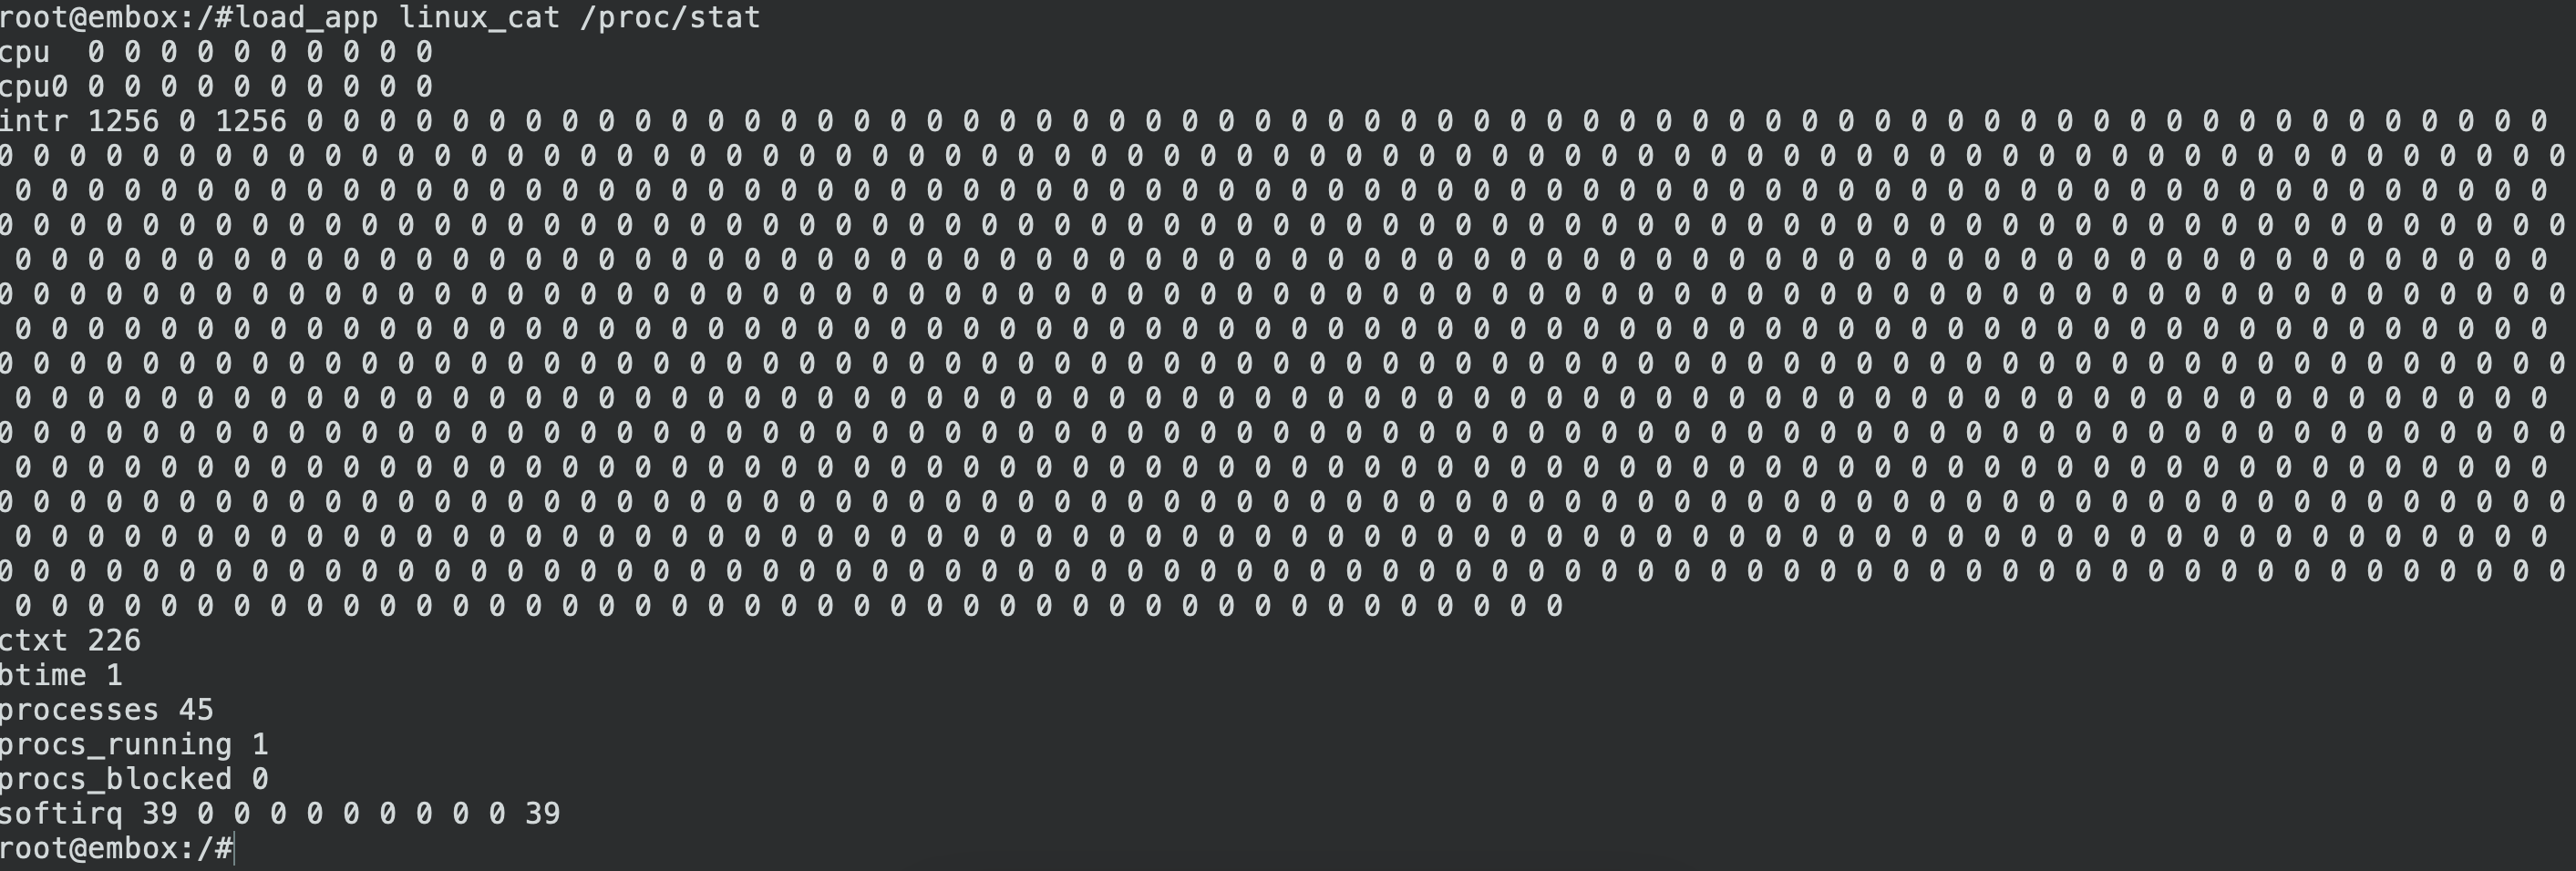
\includegraphics[scale=0.2]{pictures/embox_cat_procstat.png}}
\caption{Исполнение \textcolor{MyGrey}{\texttt{linux\_cat}} (файл \textcolor{MyGrey}{\texttt{/proc/stat}}) в ОС Embox}
\end{figure}
\end{frame}

\begin{frame}{Тестирование и апробация}
\begin{figure}[h]
\center{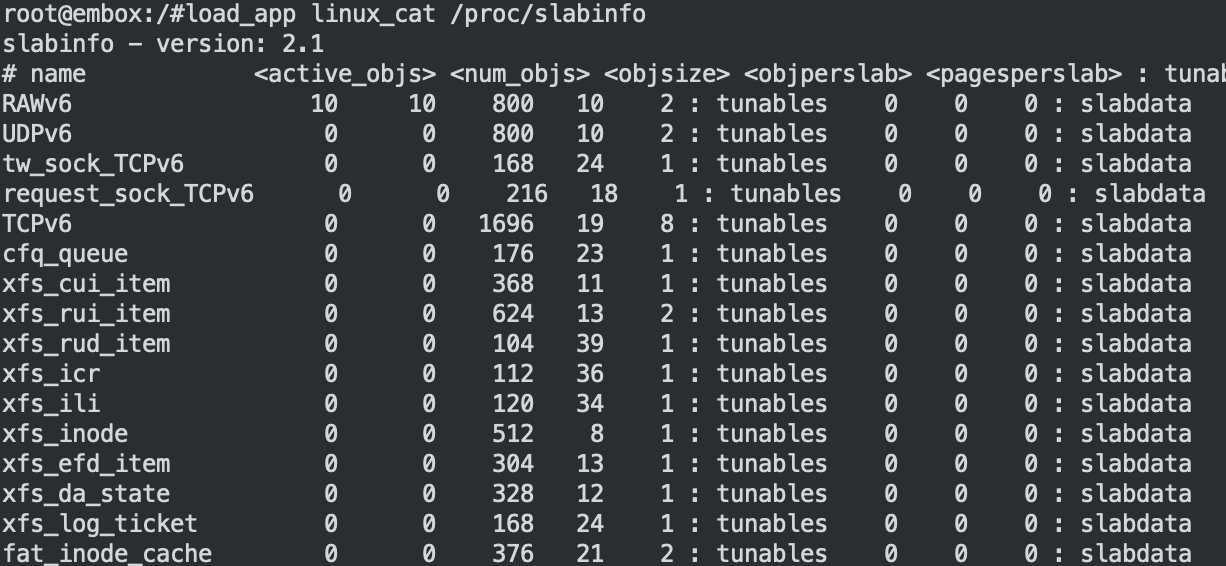
\includegraphics[scale=0.3]{pictures/embox_cat_slabinfo.png}}
\caption{Исполнение \textcolor{MyGrey}{\texttt{linux\_cat}} (файл \textcolor{MyGrey}{\texttt{/proc/slabinfo}}) в ОС Embox}
\end{figure}
\end{frame}

\begin{frame}[t]{Результаты}
\begin{enumerate}
  \item Проведён \textbf{анализ существующих подходов} к созданию двоичного слоя\newline
  совместимости с GNU/Linux в разных ОС. Выбран \textbf{метод паравиртуализации} ядра Linux.
  \item \textbf{Разработана архитектура подсистемы} двоичной совместимости с GNU/Linux, которая может быть реализована в ряде разных ОС --- это достигается за счёт использования библиотеки LKL в качестве паравиртуализированного ядра.
  \item На основе разработанной архитектуры \textbf{реализована} и настроена \textbf{подсистема для ОС Embox}.
  \item \textbf{Проведена апробация} созданной подсистемы. В Embox запущены\newline
  \textbf{демонстрационные приложения}, скомпилированные для исполнения в среде GNU/Linux. Продемонстрирована работа с \textbf{файловой системой \textcolor{MyGrey}{\texttt{procfs}}}.
\end{enumerate}
\end{frame}

\end{document}
